\section{Parte 3: Prototipos y Capturas del Sistema en Ejecución}

En esta sección se presentan y analizan los prototipos diseñados para las tres pantallas requeridas por la guía de laboratorio (\textbf{Login}, \textbf{Alertas} y \textbf{Reportes}), complementándolos y contrastándolos directamente con las evidencias del sistema real \textbf{SIGC-CUSCO} en ejecución local (\texttt{localhost:8000}).

\subsection{1. Módulo de Autenticación (Login)}
El módulo de inicio de sesión provee una interfaz unificada y accesible que permite el acceso mediante número de DNI (8 dígitos) o correo electrónico institucional, con soporte para autenticación biométrica (Passkeys/WebAuthn).

\begin{figure}[H]
    \centering
    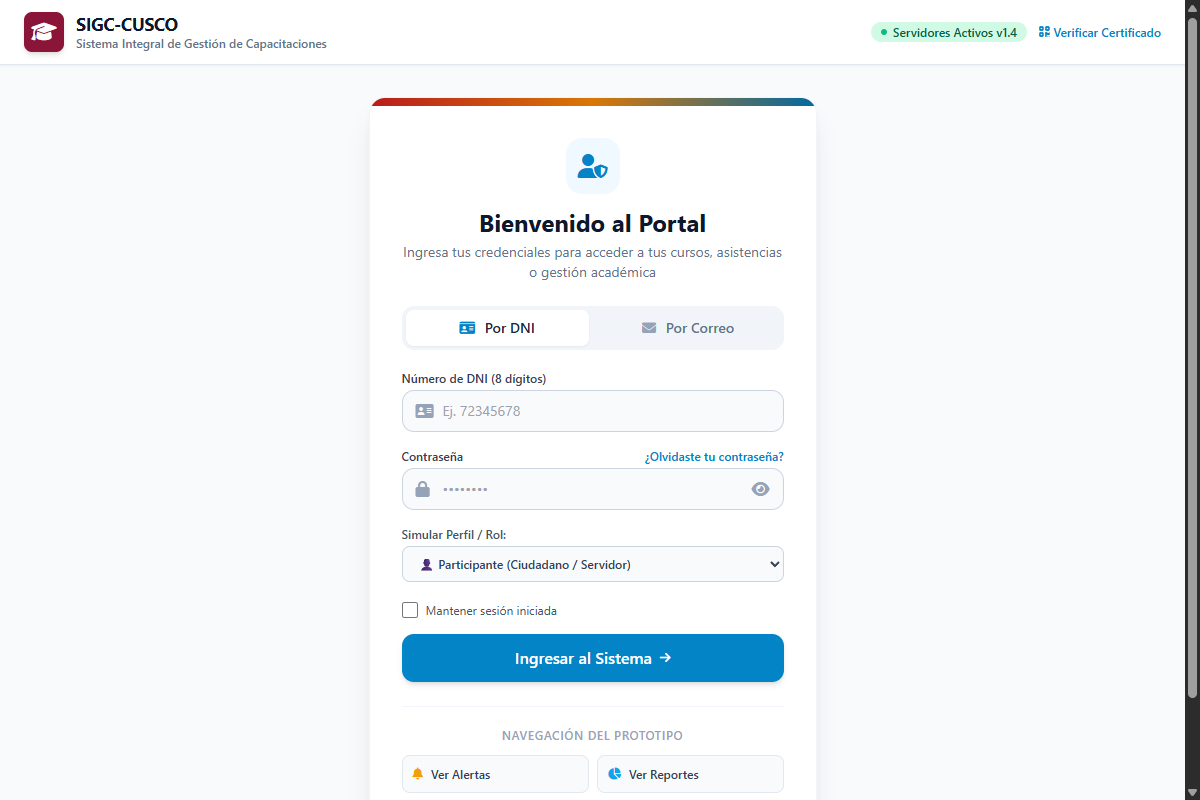
\includegraphics[width=0.88\textwidth]{pantalla_login.png}
    \caption{Prototipo de Interfaz: Inicio de Sesión (Login).}
    \label{fig:proto_login}
\end{figure}

\begin{figure}[H]
    \centering
    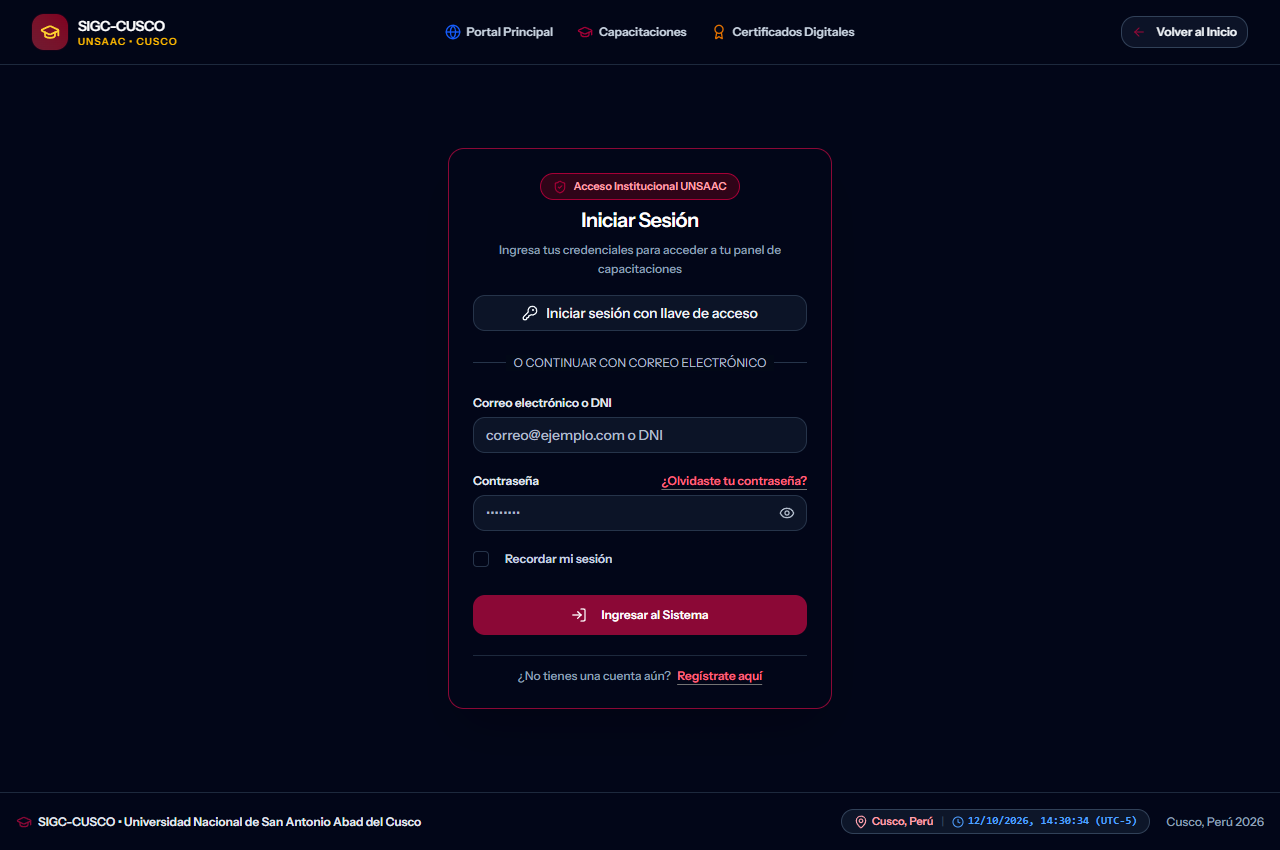
\includegraphics[width=0.88\textwidth]{sigc_real_login.png}
    \caption{Sistema Real en Ejecución: Login implementado en Laravel 13 e Inertia Vue 3.}
    \label{fig:real_login}
\end{figure}

\newpage
\subsection{2. Módulo de Alertas y Notificaciones}
El Centro de Alertas monitorea eventos críticos del ciclo de capacitación mediante códigos cromáticos estandarizados: advertencias rojas (plazo fatal de cierre de actas académicas), amarillas (riesgo de inhabilitación por 25\% de inasistencias acumuladas), verdes (emisión confirmada de certificados con hash SHA-256) y azules (proyección de sesiones con código QR).

\begin{figure}[H]
    \centering
    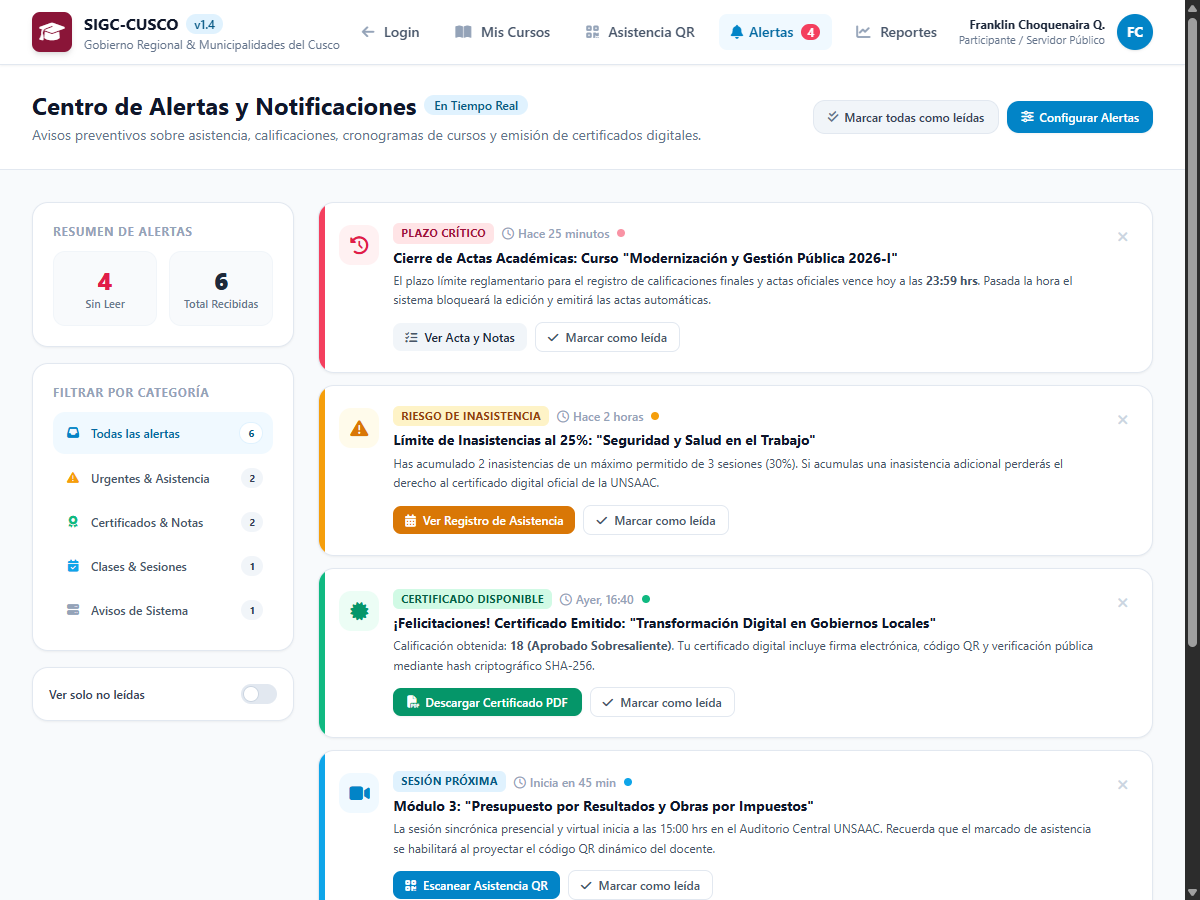
\includegraphics[width=0.96\textwidth]{pantalla_alertas.png}
    \caption{Prototipo de Interfaz: Centro de Alertas y Notificaciones Preventivas.}
    \label{fig:proto_alertas}
\end{figure}

\newpage
\subsection{3. Módulo de Reportes y Analítica Académica}
El módulo de reportes consolida los indicadores de gestión académica: tasa de asistencia por sesión, índice de aprobación, distribución de calificaciones y estado de actas oficiales. Asimismo, se contrasta con la interfaz de verificación de certificados del sistema real, donde se valida en tiempo real la autenticidad del diploma con su hash criptográfico SHA-256 verificado.

\begin{figure}[H]
    \centering
    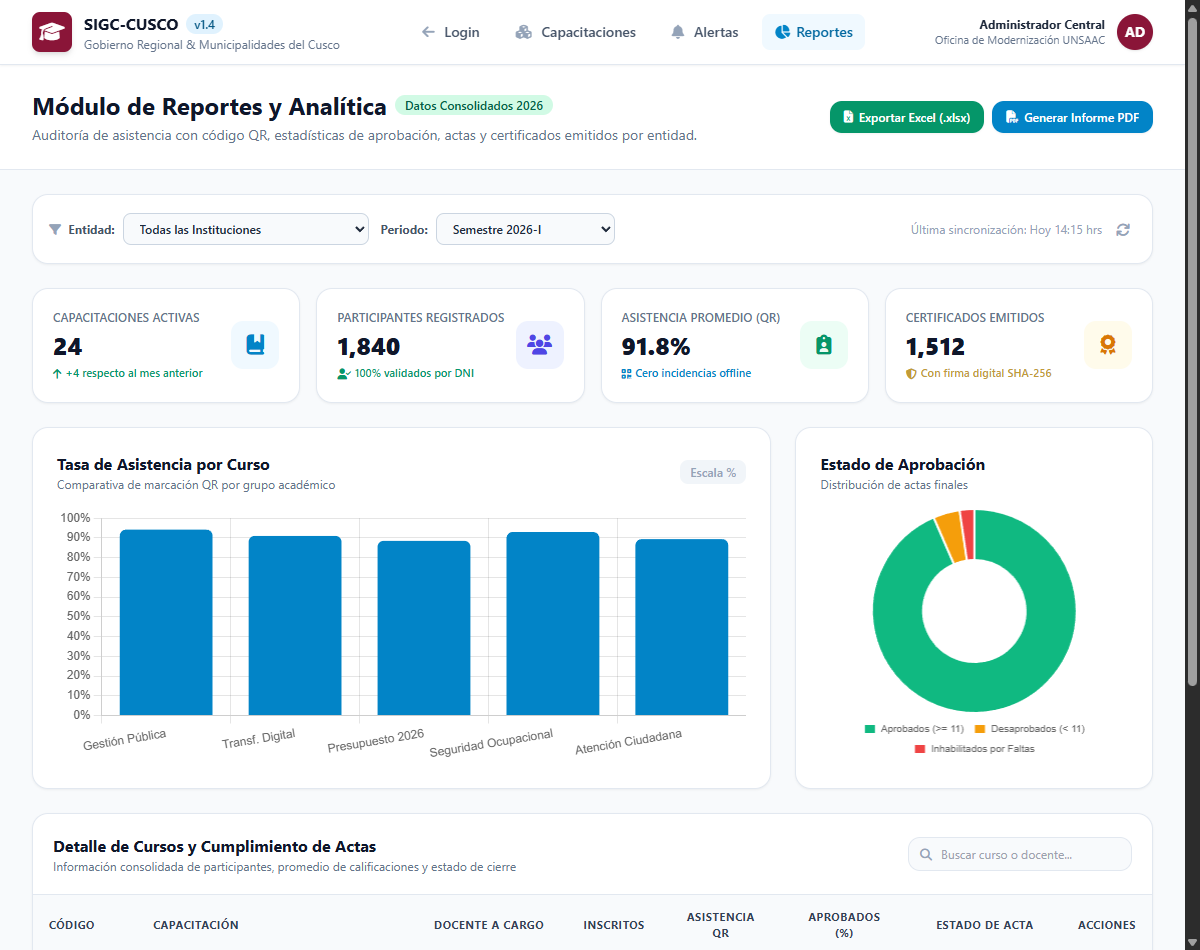
\includegraphics[width=0.94\textwidth]{pantalla_reportes.png}
    \caption{Prototipo de Interfaz: Panel de Reportes y Analítica Académica.}
    \label{fig:proto_reportes}
\end{figure}

\begin{figure}[H]
    \centering
    
\includegraphics[width=0.94\textwidth]{sigc_real_certificate_verified.png}
    \caption{Sistema Real en Ejecución: Módulo de Verificación Pública de Certificado con QR y Hash SHA-256.}
    \label{fig:real_cert_verified}
\end{figure}
